% \usepackage{graphicx}; \graphicspath{{<path to this folder>/}}

\begin{figure}[htbp]
  \centering
  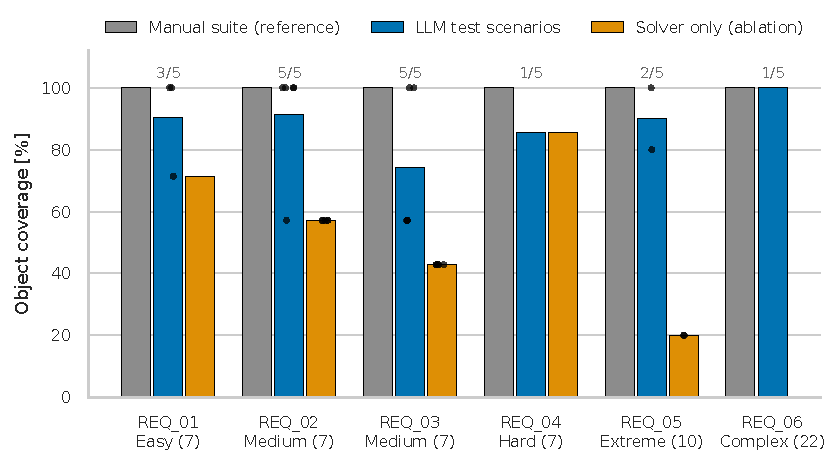
\includegraphics[width=\textwidth]{fig1_coverage_per_requirement}
  \caption{Object coverage per requirement for the manual reference suite, the LLM-designed test scenarios and the solver-only ablation (generated constraints without scenarios). Bars: mean of the successful runs; dots: individual runs; numbers above the groups: successful/all runs; in brackets: number of coverage items.}
  \label{fig:fig1-coverage-per-requirement}
\end{figure}

\begin{figure}[htbp]
  \centering
  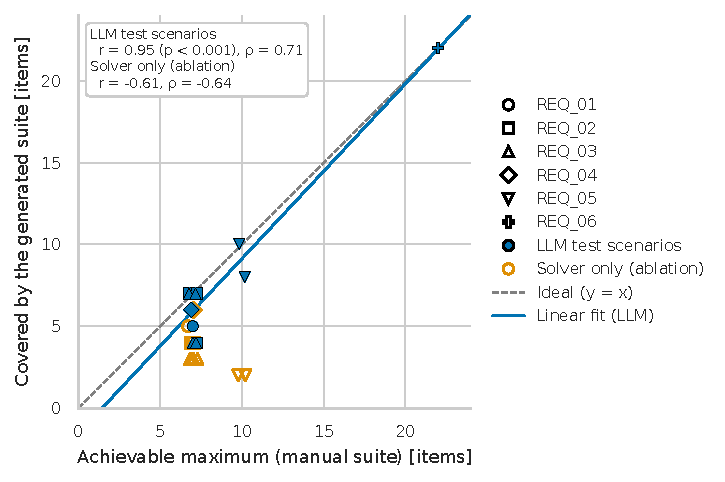
\includegraphics[width=0.85\textwidth]{fig2_correlation}
  \caption{Covered items of the generated suites versus the achievable maximum determined with the manual suite. Each point is one successful run; the dashed line is perfect agreement.}
  \label{fig:fig2-correlation}
\end{figure}

\begin{figure}[htbp]
  \centering
  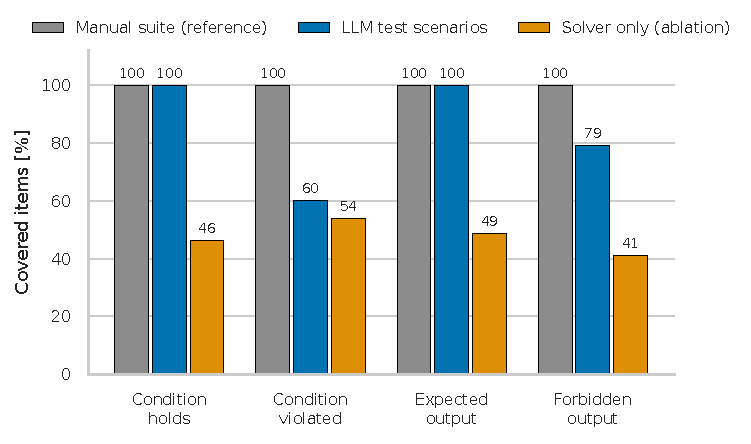
\includegraphics[width=0.85\textwidth]{fig3_item_categories}
  \caption{Coverage per coverage-item category (condition holds, condition violated, expected output, forbidden output), pooled over all requirements and successful runs.}
  \label{fig:fig3-item-categories}
\end{figure}

\begin{figure}[htbp]
  \centering
  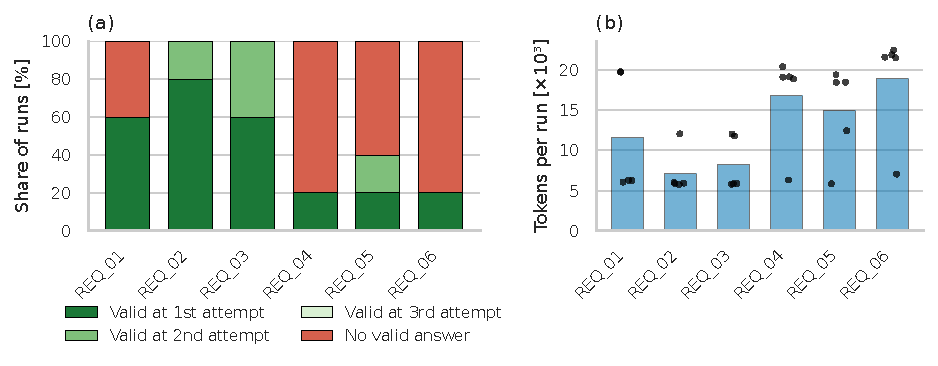
\includegraphics[width=\textwidth]{fig4_reliability_and_cost}
  \caption{(a) Outcome of the runs: the attempt at which Refinery accepted the answer of the LLM, or no valid answer after the last repair round. (b) Tokens consumed per run, summed over all repair rounds.}
  \label{fig:fig4-reliability-and-cost}
\end{figure}

\begin{figure}[htbp]
  \centering
  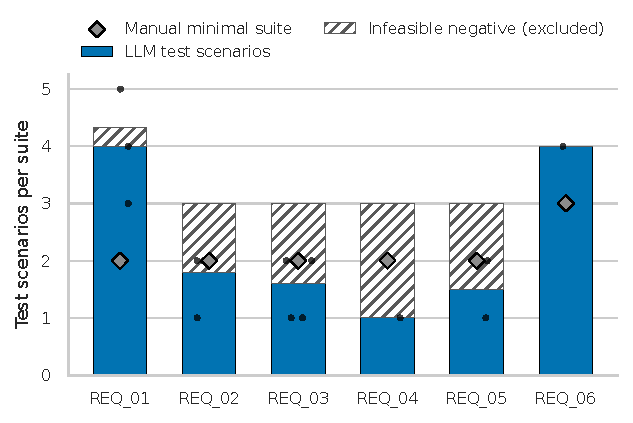
\includegraphics[width=0.75\textwidth]{fig5_suite_size}
  \caption{Number of test scenarios designed by the LLM per suite compared with the minimal manual suite. Hatched: scenarios declared as negative cases that are unsatisfiable already in the system model (without the generated constraints); they were excluded from the suite and are not counted in the coverage.}
  \label{fig:fig5-suite-size}
\end{figure}

\begin{figure}[htbp]
  \centering
  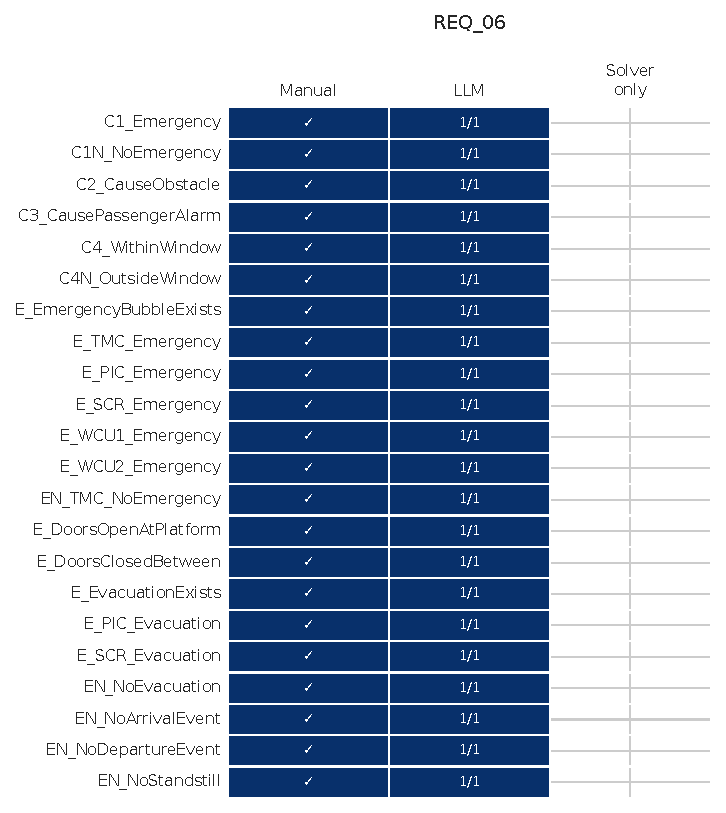
\includegraphics[width=0.6\textwidth]{fig6_items_REQ_06}
  \caption{Coverage items of REQ_06: the manual suite and the share of successful runs in which the generated suite (and the solver-only ablation) witnessed the item.}
  \label{fig:fig6-items-REQ-06}
\end{figure}
